%%%%%%%%%%%%%%%%%%%%%%%%%%%%%%%%%%%%%%%%%%%
%  Header: Document Class, Packages, and New Commands
%%%%%%%%%%%%%%%%%%%%%%%%%%%%%%%%%%%%%%%%%%%

\documentclass[conference]{IEEEtran}

\usepackage{booktabs}
\usepackage[usenames,dvipsnames]{xcolor}
\usepackage[normalem]{ulem}
\usepackage{pifont}
\usepackage{multirow}
\usepackage{graphicx}
\usepackage{makecell}
\newcommand{\urlwofont}[1]{\underline{\urlstyle{same}\url{#1}}}

\newif\ifrev
%  COMMENT OUT NEXT LINE TO HIDE TODOs AND COMMENTS
\revtrue

\ifrev
  \newcommand{\yanyan}[1]{{\color{blue} [Yanyan: #1]}}
  \newcommand{\cappos}[1]{{\color{red} [Justin: #1]}}
  \newcommand{\lois}[1]{{\color{magenta} [Lois: #1]}}
  \newcommand{\yiwen}[1]{{\color{OliveGreen} [Yiwen: #1]}}
  \newcommand{\todo}[1]{{\color{Orange} [TODO: #1]}}
\else
  \newcommand{\yanyan}[1]{}
  \newcommand{\cappos}[1]{}
  \newcommand{\lois}[1]{}
  \newcommand{\yiwen}[1]{}
  \newcommand{\todo}[1]{}
\fi

%%%%%%%%%%%%%%%%%%%%%%%%%%%%%%%%%%%%%%%%%%%
%  Begin of Document
%%%%%%%%%%%%%%%%%%%%%%%%%%%%%%%%%%%%%%%%%%%

\begin{document}

%%%%%%%%%%%%%%%%%%%%%%%%%%%%%%%%%%%%%%%%%%%
%  Title and Authors
%%%%%%%%%%%%%%%%%%%%%%%%%%%%%%%%%%%%%%%%%%%

\title{Lind: Shielding Privileged Code From Untrusted Programs 
Through Controlled Kernel Access}

\author{\IEEEauthorblockN{Yiwen Li}
\IEEEauthorblockA{New York Univeristy \\
Email: liyiwen@nyu.edu}
\and
\IEEEauthorblockN{Ali Gholami}
\IEEEauthorblockA{KTH Royal Institute of Technology \\
Email: gholami@kth.se}
\and
\IEEEauthorblockN{Chris Matthews}
\IEEEauthorblockA{Apple \\
Email: chris.matthews@apple.com }
\and
\IEEEauthorblockN{Yanyan Zhuang}
\IEEEauthorblockA{New York University \\
Email: yyzh@nyu.edu}
\and
\IEEEauthorblockN{Justin Cappos}
\IEEEauthorblockA{New York University \\
Email: jcappos@nyu.edu}
}

\maketitle

%%%%%%%%%%%%%%%%%%%%%%%%%%%%%%%%%%%%%%%%%%%
%  Abstract
%%%%%%%%%%%%%%%%%%%%%%%%%%%%%%%%%%%%%%%%%%%

\begin{abstract}

Building secure systems that allow untrusted programs to run without
triggering vulnerabilities in the underlying privileged code of an
operating system (OS) kernel or hypervisor is very challenging. \yanyan{sentence too long}Despite
substantial effort by security researchers and system developers to
eliminate these flaws, exploitable vulnerabilities can still be found.
Techniques to protect against intentional or unintentional triggering of
these vulnerabilities, such as system call filtering, operating system
virtualization, and library OSes have had limited success.  The problems
of these techniques are two-fold.  First, these systems add trusted code that often has new
exploitable vulnerabilities. Second, the portions of the underlying kernel
that these systems use may enable the attacker to exploit vulnerabilities.
As a result, they can not fully prevent buggy programs from triggering
flaws, or attackers from leveraging these bugs. 
%for their own purposes.

\cappos{Rework...}
In this paper, we introduce a novel security design that leverages
controlled kernel access to protect privileged code from exploitation by
untrusted programs. We start by analyzing the effectiveness of existing
solutions and explore the reasons why existing techniques are not
effective. We then present a new metric to determine where kernel flaws are
likely to be located, based on a hypothesis that commonly-used kernel
paths, executed by applications on a daily basis, contain fewer
vulnerabilities than less-used paths. Next, we use this insight to devise a
novel design that reimplements \yanyan{replace reimplement with 
something else?} essential OS functionality inside a
sandbox that only accesses commonly used kernel paths. Lastly, we use this
design to prototype a security system called Lind. Our
experiment results show that an attacker executing code inside Lind can 
trigger less than 3\% of zero day kernel attacks, which is about an order of
magnitude less than existing systems like VirtualBox (40\%), VMWare
Workstation (31\%), Docker (23\%), and Graphene (23\%).  


\end{abstract}


%%%%%%%%%%%%%%%%%%%%%%%%%%%%%%%%%%%%%%%%%%%
%  Sections
%%%%%%%%%%%%%%%%%%%%%%%%%%%%%%%%%%%%%%%%%%%

\section{Introduction}
\label{sec.introduction}

To run multiple applications on a computer, it is critical to securely
manage access to the underlying hardware. In modern computer systems,
either a hypervisor - a virtual machine monitor (VMM), or an 
operating system (OS) kernel performs this important function. Unfortunately, code within an OS kernel may contain flaws and vulnerabilities. If the OS kernel is attacked by a malicious adversary, potential vulnerabilities can enable the attacker to have unrestricted access to the system.


%One critical flaw, discovered in the Linux kernel in the \texttt{futex} subsystem call can allow an attacker to gain ring 0 control via the \texttt{futex} syscall, and potentially execute arbitrary code with kernel mode privileges~\cite{CVE-2014-3153}. \cappos{Possibly omit this sentence.}


There is a diverse set of defensive technologies to protect kernels from 
attacks, including OS virtualization \cite{Xen-03},\cite{Microsoft-Hyper-V}, system call filtering \cite{Janus0:96, Janus:99},\cite{SCI-04}, and library OSes \cite{Bascule},\cite{Drawbridge-11},\cite{Graphene-14}. Common security wisdom is that by running software in a virtual machine, 
one can prevent the attacker from exploiting flaws in the underlying kernel.  However, the security of virtualization itself is a 
challenging issue \cite{Tal}. As we will show later, virtualization cannot prevent about one third of vulnerabilities on the Linux kernel. As such, even with these technologies in place, applications running in a virtual machine still pose a substantial risk.

In this paper, we first develop a metric that helps identify where
within the kernel these vulnerabilities are likely to be located. We
examined 40 kernel patches that fix severe Linux kernel security bugs
and analyzed the lines of the kernel where those bugs occurred.  Our
analysis shows that kernel paths used by popular applications contain fewer
security bugs, and therefore, can be exposed with less risk. 

While limiting access to kernel code is important, it is
insufficient to build a secure virtualization system.  First, if a complex
program is prevented from accessing part of the kernel, its functionality 
must exist somewhere else for this program to work.  Second, it is 
typical for virtualization systems to add new privileged code.
As a result, a vulnerability in the privileged codebase is as much of a security 
risk as a flaw in the kernel.  %However, this privileged code needs to be
%complex because the system must implement complex 
% must exist somewhere or else applications will not run. 
For example, 
a vulnerability in VMWare's codebase caused by buffer overflows in the VIX
API could allow local users to escape out of the guest VM and 
gain privilege escalation to execute arbitrary code in the host
OS, even shellcode to access the kernel of the host OS~\cite{CVE-2008-2100}.  
%\cappos{Revise this paragraph further}
\cappos{We need an example of a root exploit in the host OS being triggered 
from a guest...  This is just a guest escape...}

%To address this issue, 
We propose a new design paradigm for virtualization 
systems called ``safely-reimplement'' that restricts access to only the
kernel paths that are mostly used by common applications.  To restrict the privileged
code, we first build a minimal, sandboxed environment that also only uses 
common kernel paths.
We then implement a POSIX interface inside of this safe sandbox. For complex and dangerous system functions, which may access the risky portion of the kernel, 
input to POSIX is reimplemented by our own code within a sandbox. Any bugs or failures within the implementation of those complex system functions 
will be contained by the sandbox, and will not have the chance to reach 
and trigger risky portions of the kernel. Because of this added security, we dub this as a "safe-reimplementation" design. \yanyan{the sandbox only has
safe code. how can unsafe code to be trapped "within" the sandbox?} Therefore, even if the code
is vulnerable to an attack, it is unable to trigger
kernel paths that are less commonly used or tested.

This implementation helped us to understand which kernel paths are hardest to
safely-reimplement and provided key insights about what kernel paths system
designers should give the highest degree of scrutiny. In turn, we then use this design paradigm to develop a virtualization system called
Lind.  Lind uses Google Native client for software fault isolation (memory
safety of the application) and the Repy sandbox~\cite{Repy-10} to contain the POSIX
implementation and to provide access to the kernel.   \yanyan{shouldn't it
be the other way round? first fully understand which paths are hard, and
then use this insight to design Lind.}

To evaluate the effectiveness of Lind, we first captured the 
kernel traces from user programs run in Lind and four other virtualization
systems.
%and compare their kernel traces. 
We then examined historical
kernel bug reports to verify which trace was more likely to trigger bugs.
Results showed that applications run in Lind were the least likely to
trigger kernel bugs: only one triggered out of the 35 kernel vulnerabilities 
(2.9\%). In contrast, the virtualization systems built
without our metric triggered more vulnerabilities (23-40\%). This
suggests that our metric can help effectively design and build more secure
virtualization systems.

The main contributions of this paper are as follows: %\cappos{revise}
\begin{itemize}
\item We propose a novel metric for quantitatively measuring and evaluating the
security of privileged code, such as in an OS kernel. Our metric examines
the safety of the kernel trace, at the lines-of-code level, generated by
running user applications. This metric is helpful for the design of secure systems.
%\yanyan{what is "generated by producing design recommendations"?}
\item Using our metric, we have substantiated our key hypothesis that commonly
used kernel paths contain fewer bugs. 
\item We create a novel secure ``safely-reimplement'' design by examining and
leveraging our metric and key hypothesis. 
%that commonly used kernel paths contain fewer bugs. 
Our design reimplements risky system calls inside a
sandbox that only uses safe kernel paths. 
\item With this new design, we implemented a sandbox security system, Lind, that
provides a secure environment for applications and strong protection for
the kernel.
\item Results show that the implementation of Lind only triggers one (2.9\%) of
the kernel vulnerabilities we examined, while systems built without using
our metric trigger about an order of magnitude more vulnerabilities. This
suggests that our metric can help design and build virtualization systems
with greater security. 
\end{itemize}
\cappos{Quantitative analysis for sandboxes}


The remainder of this paper is organized as follows. 
We discuss the motivation that drove our work and key background information 
in \S{\ref{sec.motivation-and-background}}. 
In \S{\ref{sec.metric}}, we propose our kernel coverage safety metric. 
%to solve the existing security problems.  
Using this metric, we describe the 
``safely-reimplement'' design pattern in \S{\ref{sec.design}}. In 
\S{\ref{sec.implementation}}, we describe the sandbox security 
system Lind, which is implemented using our design. We use quantitative 
measures to compare the security and efficiency of Lind with other 
virtualization systems in \S{\ref{sec.evaluation}}. 
Limitations and future work are discussed in \S{\ref{sec.limitation}}.  
We then discuss related work in \S{\ref{sec.related_work}} and conclude
in \S{\ref{sec.conclusion}}.


\section{Motivation and Background}
\label{sec.motivation-and-background}

This section presents background information 
relevant to the development of our design metric and the Lind prototype and threat assumptions. The problem of kernel exploitation and the limitations of previous protection strategies also have been briefly discussed. 
%caused by an inability to identify which portions of the kernel are risky. 

\subsection{Kernel and Vulnerabilities}

Running user applications relies on the operating system kernel 
accessing critical resources, such as memory, I/O, or CPU. 
The kernel provides interfaces to serve these requests 
and provides essential functionality for all applications running in the
system. 
Thus all code, whether sandboxed or untrusted, will make calls 
that are eventually processed by the kernel. 

Unfortunately, the OS kernels are not safe and secure against adversarial attacks that is worsening over time. Over the past few years, exploitation of the OS kernels has been wide
spread, despite substantial efforts by researchers and practitioners. 
In 2014, 215 vulnerabilities in all types of kernels were reported~\cite{NVD}, 
and 125 of those vulnerabilities were related to the Linux kernel. 
The kernel's
attack surface keeps increasing due to the constant addition of new
features~\cite{Metrics-13}. For example, the Linux kernel grew from 6.6 MLOC in v2.6.11 (March 2005) to 16.9 MLOC in v3.10 (June 2013)~\cite{Linux-13}. 

\cappos{Likely cut this.  I think it is excessive.}

Such a huge kernel codebase has lead to excessive exploitation, where it has been plagued by a number of common
software flaws. 
These flaws have raised serious security concerns and caused severe damage
to systems. 

The common vulnerability and exposure (CVE) database reports indicate stack and heap buffer overflow vulnerabilities have been used to launch denial of service attacks through crashing the systems (CVE-2013-2892).
%~\cite{CVE-2013-2892}, 
Other vulnerabilities such as the execution of arbitrary code (CVE-2009-3234) 
%~\cite{CVE-2009-3234}, 
or to allow local users to gain privileges via a crafted 
application (CVE-2013-1828) are also among the reports.
%~\cite{CVE-2013-1828}. 
Memory disclosure vulnerabilities (CVE-2009-3002) have been also exploited to allow local users
to read 
the contents of some kernel memory locations
%~\cite{CVE-2009-3002}
, or to obtain potentially sensitive information from kernel stack memory (CVE-2010-4073).
%~\cite{CVE-2010-4073}. 
Attackers have also used use-after-free vulnerability to gain kernel
privileges, i.e. CVE-2013-4343.
%~\cite{CVE-2013-4343}.

%The number of kernel vulnerabilities and their potential for exploitation, 
%plus the fact that user applications rely on the kernel to execute
%programs, 
%present a compelling motive for designing securer systems that can run
%applications with a better degree of safety. \yanyan{this paragraph does 
%not say anything new.}

\subsection{Threat Assumptions}

The primary goal of a secure system is to restrict a program to some subset
of privileges, 
usually by exposing a set of functions that mediate access to the
underlying operating system privileges. 
Threats occur when applications obtain access to privileges that were not
intentionally granted by the system, 
thus losing the intended protection~\cite{Repy-10}. To apply the proposed security metric to a developing system, we make the following assumptions:

\begin{enumerate}
\item The OS kernel contains at least one bug that is known to an adversarial attacker.

\item The attacker has the ability to execute code inside
of a virtualized system, such as an operating system VM or library OS.
The attacker may either have that access by writing a malicious application
that the user executes or by exploiting a flaw that exists in a user's
application.

\item Unintentional bugs will exist in any complex code. This
includes any security systems placed between the kernel and the user
applications.

\item Feasibility to provide some form of computational 
containment. This means that an isolated program cannot simply
make arbitrary system calls and access the kernel directly. This could
be provided through software-fault isolation~\cite{SFI:93}, programming 
language techniques\cappos{cites}, or by running isolated code in a
distinct region of virtual memory\cappos{cites}.

\item Possibility to build functionality that possesses few
vulnerabilities as long as it keeps the code-base to a minimum.

\cappos{How do I explain
the sandbox TCB???  How is this different from a hypervisor?}

\end{enumerate}


\section{Developing and Assessing a Quantitative Evaluation Metric for
Kernel Security}
\label{sec.metric}


In this section, we describe in detail the aforementioned metric to 
quantitatively evaluate kernel security. We first discuss issues with
commonly used metrics for code complexity. Then we present our metric that
focuses on using kernel code paths used by common applications.  We
then show how our metric is able to provide a fair comparison of 
different security systems, their impact on the kernel, 
and to reveal which portions contained fewer bugs.

\subsection{Previous Risk Metrics for Software}

A contributing factor to the kernel security problem is that system
designers 
still lack a standard method for quantifying the safety (or risk) of
privileged code.   \cappos{Is this really true?  No one has ever proposed
a metric?  We do need to do a more detailed analysis of this.  I would vote
to remove this sentence regardless...}

Researchers have studied and explored different metrics to identify and
predict bugs in software systems. 
The number of lines of code has been used as one 
predictor~\cite{Bug-Location}, as has a file's revision status and 
whether or not the file previously contained bugs~\cite{Bug-Location, 
lewis2013does}. Studies have also been done based on 
the number of functions and/or the number of executable lines of code in
the function~\cite{Mining-Metrics}. 
While these metrics can be useful in building models to provide a general
idea about 
where bugs may be located in software systems, they have limitations. 
Firstly, the metrics mentioned above are not specifically designed for
studying bugs in OS kernels. 
\cappos{Why does this matter?}
Therefore, they do not take into account the way system calls are invoked
by user applications. 
Moreover, these metrics can not provide information about the accurate
location of the bugs within the kernel, 
which is important to our study.
\cappos{Are you going to show that this is true?  Can you explain more
about why these do not work?}
\cappos{Do existing metrics work on a LOC level?  }

Without any type of guidance as to what parts of the kernel are safe, past
initiatives, 
such as building a sandbox or using library OSes, could only focus on
isolating user programs.  \cappos{What are you saying?}
These methods can mitigate the problem, but the proposed systems will still
access the kernel the same way as before. 
They simply move the attack surface from between the user space and the
kernel, \yanyan{what's the purpose/consequence of this move? why is this
move good or bad?}
to between these new systems and the kernel, but the surface is not
necessarily reduced. 
As a result, the proposed solutions do not make the systems more secure. 

Recognizing this limitation, we proposed a novel security metric to
quantitatively measure and evaluate the kernel: 
checking kernel coverage safety at the level of lines of code against
existing kernel bugs. 
With this metric, we would be better able to understand security features
of the kernel, 
and design an interface that is exposed to the user space in a secure way.
Ideally, 
this would mean only exposing the safe portions of the kernel to the user
space. 
However, in some cases, risky portions must be exposed to the kernel as
well. 
The kernel coverage safety metric, however, can provide us a guidance 
about the potential dangers and 
can help us safely-reimplement those risky kernel interface (or system
calls) to avoid the potential damage.
%\yanyan{I don't think the new metric alerts us tho. maybe say it provides 
%as a guidance which parts are risky?}




\cappos{end of text}





\subsection{Key Hypothesis}

Our hypothesis is that kernel paths executed by popular applications, 
such as Web browsers, or file editors, are likely to contain fewer
exploitable bugs 
than uncommonly used paths. Our reasoning is that, because they are
frequently used, 
bugs and vulnerabilities in these common kernel paths
would have most likely been caught by developers. 
Note that this does more than indicate which system calls should be used. 
A metric that looks at commonly used kernel paths also excludes odd
execution paths 
through popular system calls. 
This means that the chances to harbor kernel bugs in those commonly used
kernel paths are slim. 

The procedure for testing the hypothesis is described, and the results
discussed, in the following sections. 

\subsection{Foundation for the Metric: Capturing and Evaluating Kernel
Traces}

The first step in proving our hypothesis was to capture the lines of kernel
code executed 
when running applications. The OS kernel code is organized under different
kernel directories. 
Whenever an application tries to access system resources, such as file
system I/O and memory, 
the kernel code under the corresponding paths is executed. Therefore, 
its code execution reflects the basic behavior of the kernel, in response
to user application requests. 
Our metric first identified and captured which lines of code in the kernel
were executed 
when running an user program. We named the resulting captured lines of
code a \textit{kernel trace}. 
A kernel trace is closely related to the program that generated the trace. 
By using the kernel traces, a comparison between different
security systems is possible. 
To capture the kernel trace, we used \texttt{gcov} \cite{gcov}, a program profiling
tool that is a standard utility with the GNU Compiler Collection (GCC) suite. 

The second step was to evaluate security aspects of the kernel traces that
we captured. 
Using the historical kernel vulnerability reports, we collected a list of
severe kernel bugs from 
the National Vulnerability Database, the U.S. government repository of
standards-based \yanyan{what does standards-based mean?}
vulnerability management data \cite{NVD}. We analyzed the bugs as
follows. For each bug, we identified the lines of code 
in the kernel that would trigger it. This can be done by examining 
a patch of the Linux kernel source code to fix the bug. From the patch, 
we can identify \textit{which lines of kernel code need to be modified in order to
remove the bug}. 
A user program that executes the lines of code changed by a patch to fix a
kernel bug is considered to have the \textit{potential to exploit that flaw}.

We determined that the lines of code in the kernel would be risky 
if they triggered one or more kernel vulnerability, and those lines of code 
that did not are considered to be safe. Using the above kernel trace
analysis, 
we empirically labeled the lines of code in the kernel that contain fewer
bugs as safe lines. \yanyan{according to the definition, safe lines should
contain no bug, instead of fewer bugs.}
The safe lines of code would then compose the safe portion of the kernel, 
which can be trusted to build a secure trusted computing base for secure
systems.

\subsection{Verification of Hypothesis}

To verify our hypothesis that commonly used kernel paths contain fewer bugs, 
we identified these paths as a subset of the total reachable kernel
paths as follows:

%\begin{enumerate}
First, common paths were captured by running popular user applications or open-source libraries. Most notably, these experiments were conducted in data collection phase included running several applications such as two large-scale browsers (Mozilla Firefox and Google Chrome), in addition to running 50 packages among the top 200 popular Debian packages \cite{Top-Packages} in a Linux kernel version 3.13.0.
\cappos{What version of Linux?}  \cappos{Ali: why these apps?}

In this step, several other experiments that were required to be completed such as intensive file management tasks to create/read/update or delete files and directories from the underlying (ext3) filesystem during a discrete period of 20 hours over 5 days.
\cappos{This all needs to be much better explained...}

Next, the total reachable paths were required to be captured by comprehensive system call fuzzing and running the Linux kernel test suite. This experiments helped to capture the total reachable paths in the kernel as completely \gholami {thoroughly?} as possible. 

Two approaches were used to capture this trace.

\begin{itemize}
\item The system call fuzzing experiment were designed to utilize the Trinity system call fuzz tester \cite{Trinity}. This included sequential execution of more than 300 system calls with 1 million iterations for executing each system call by 16 child processes as Trinity workers.

The including file management and network system calls, \yanyan{what is file management?} which gave us a thorough kernel trace. 

\item Linux Test Project (LTP) \cite{LTP} was another tool that was used to capture the total reachable kernel trace.

\cappos{Why did we do this?  Was this to validate our results?  Did it work?
Did the test show anything separate from fuzzing?}
Linux Test Project is a mature and well maintained tool to test the Linux
kernel. 
We ran all the available system call test cases with this tool to capture
the kernel trace. 
\end{itemize}
%\end{enumerate}

Combining the kernel traces generated by Trinity and LTP, we were able to
access our total reachable kernel paths.
We found that 38.5\% of the total reachable
kernel paths are commonly used. 
More importantly, only 2.5\% of the bugs examined were found in the common
paths, 
while 50\% of the bugs were found in the total reachable kernel paths. 
Our results confirm that common paths contain fewer bugs than uncommon
paths. \yanyan{I feel this is a bit early to make this conclusion.}

\subsubsection{Coverage Analysis of Common Paths}

The kernel trace coverage of the common paths and the total reachable paths
are shown in Table \ref{table:kernel_coverage}. 
The results show that the size of commonly-used kernel paths is small,
merely 12.4\% of the entire kernel code base. 
The common paths coverage is also significantly smaller than the total
reachable paths coverage 
(about 1/3 of the entire kernel).

It may appear surprising that the total reachable paths coverage is low, 
and accounts for only about one-third of the entire kernel.  However, 
this is consistent with kernel code coverage analysis 
measurements conducted by other researchers \cite{LTP-Coverage}.
One reason that this occurs is that many paths 
in the kernel cannot be accessed from the system call API. Another reason
is that 
while obtaining the kernel coverage data, as most researchers did, we used
a system call fuzzing tool 
and a Linux test suite to generate the kernel trace. The existing fuzzing
tools and test suite do not reach every possible path in the kernel.
\cappos{Why?}

%Although the total reachable paths coverage is not 100\% of the entire
%kernel code base, 
%it is still very large and contains many bugs. 
%However, because the commonly used kernel path coverage is much smaller
%than 
%the total reachable path coverage, this is a positive indication that these
%relatively small areas can be considered safe.

\begin{table}
\centering
\scriptsize
\caption {Kernel Coverage}
\begin{tabular}{|l|c|}
  \hline
  \textbf{Kernel Paths} & \textbf{Kernel Coverage (percentage)} \\
  \hline \hline
  Common Paths & 12.4\% \\
  \hline
  Total Reachable Paths & 32.2\% \\
  \hline
\end{tabular}
\label{table:kernel_coverage}
\end{table}

The results from Figure \ref{fig:subset} and Figure
\ref{fig:key_paths_trace}  \cappos{What do these actually mean?}
show that the common paths are a subset of the
total reachable paths, 
shown by the ``OverlappedLines'' in Figure \ref{fig:subset} and Figure
\ref{fig:key_paths_trace}. 
We closely examined the kernel trace derived from common paths
and the total reachable paths. We found that for each different path
in the kernel, the lines of code 
in the common paths trace also appeared in the total reachable paths trace.
But there are many lines of code (more than 50\%) 
in the total reachable paths trace that are not in the common paths. This
shows that the common paths trace and 
the total reachable paths we obtained are correct, because common paths in
the kernel should definitely be reachable. \yanyan{how to define correct?}
One further finding is that the common paths account
for only 38.5\% of the total reachable paths. 
This suggests that a large portion (61.5\%) of the kernel is not frequently
used by popular applications on a daily basis.

\begin{figure}
\centering
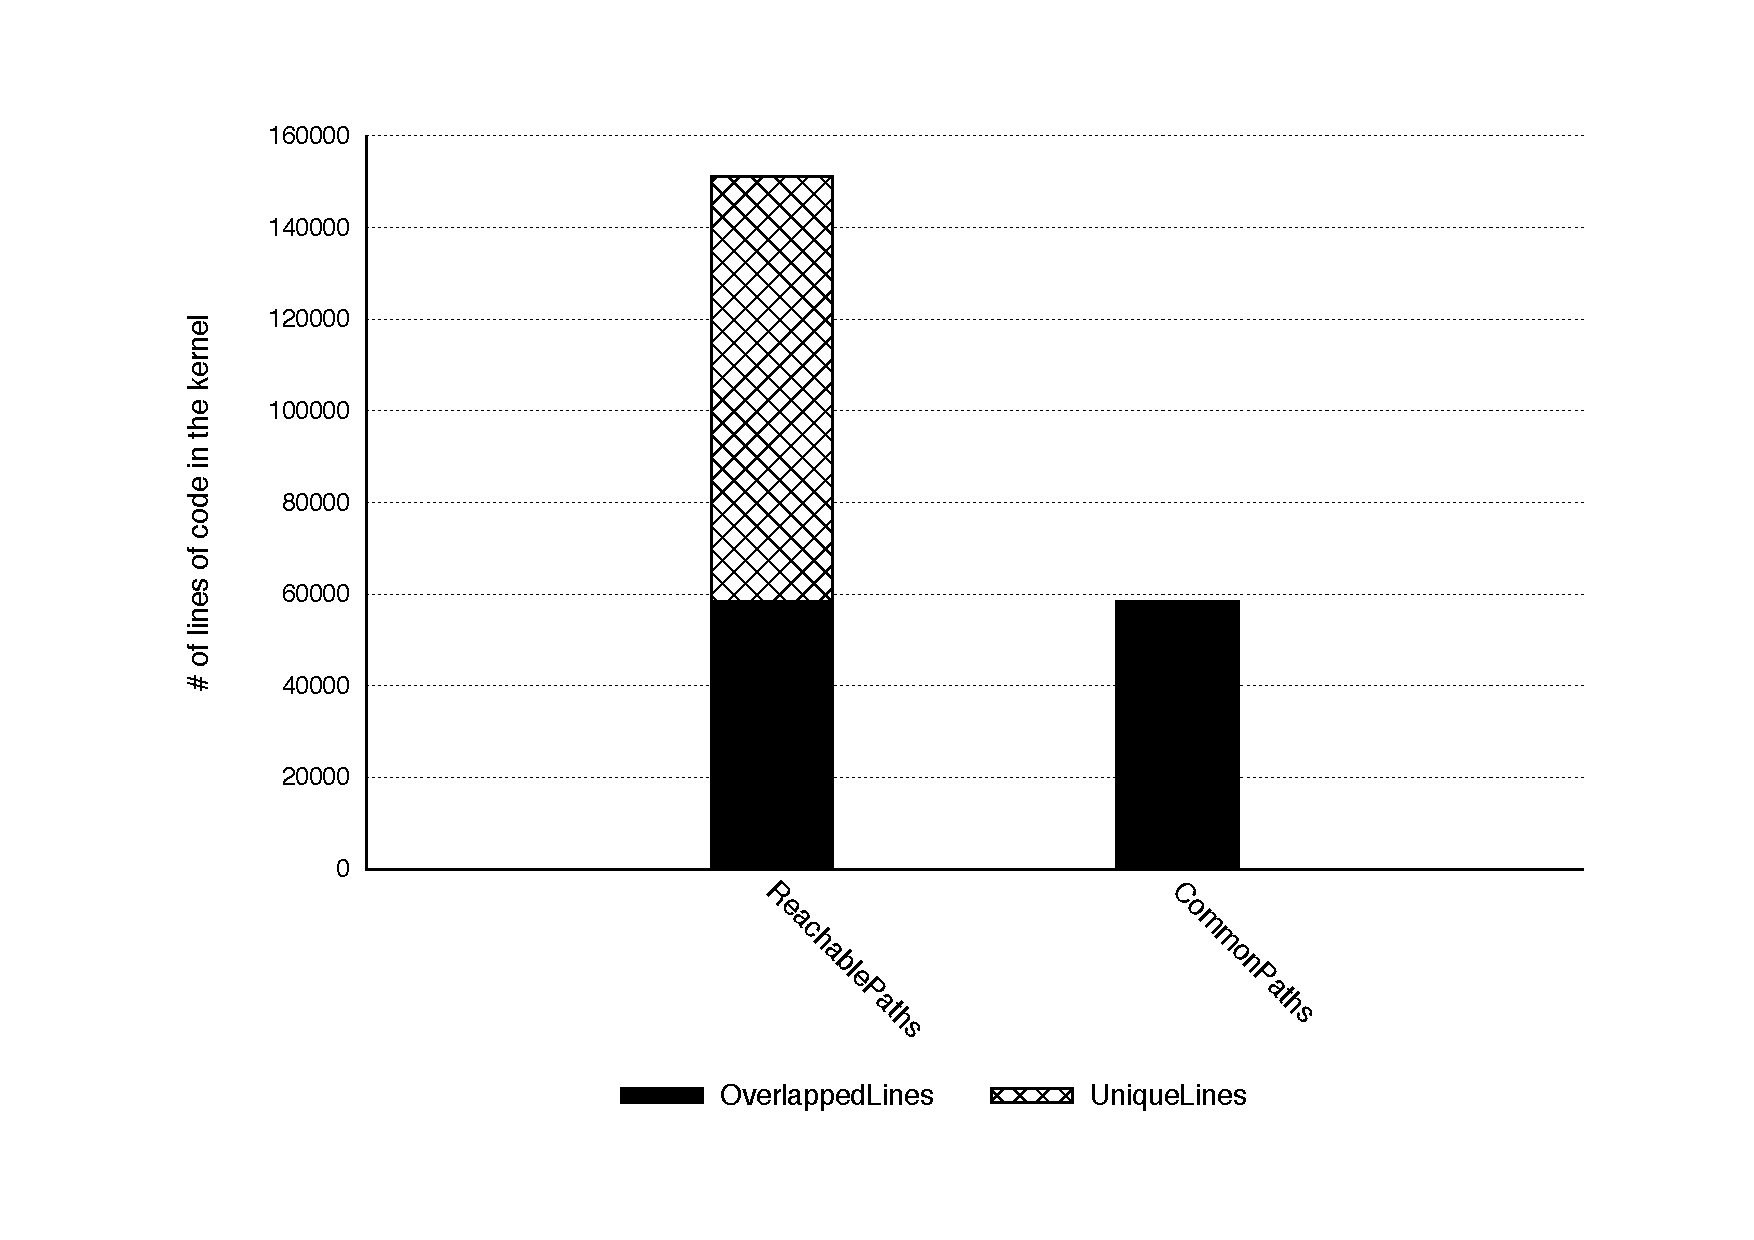
\includegraphics[width=1.0\columnwidth]{diagram/lind_oakland16_diagram_01.pdf}
\caption{Kernel Trace Comparison: Common Paths as a Subset of Reachable
Paths}
\label{fig:subset}
\end{figure}

\begin{figure}
\centering
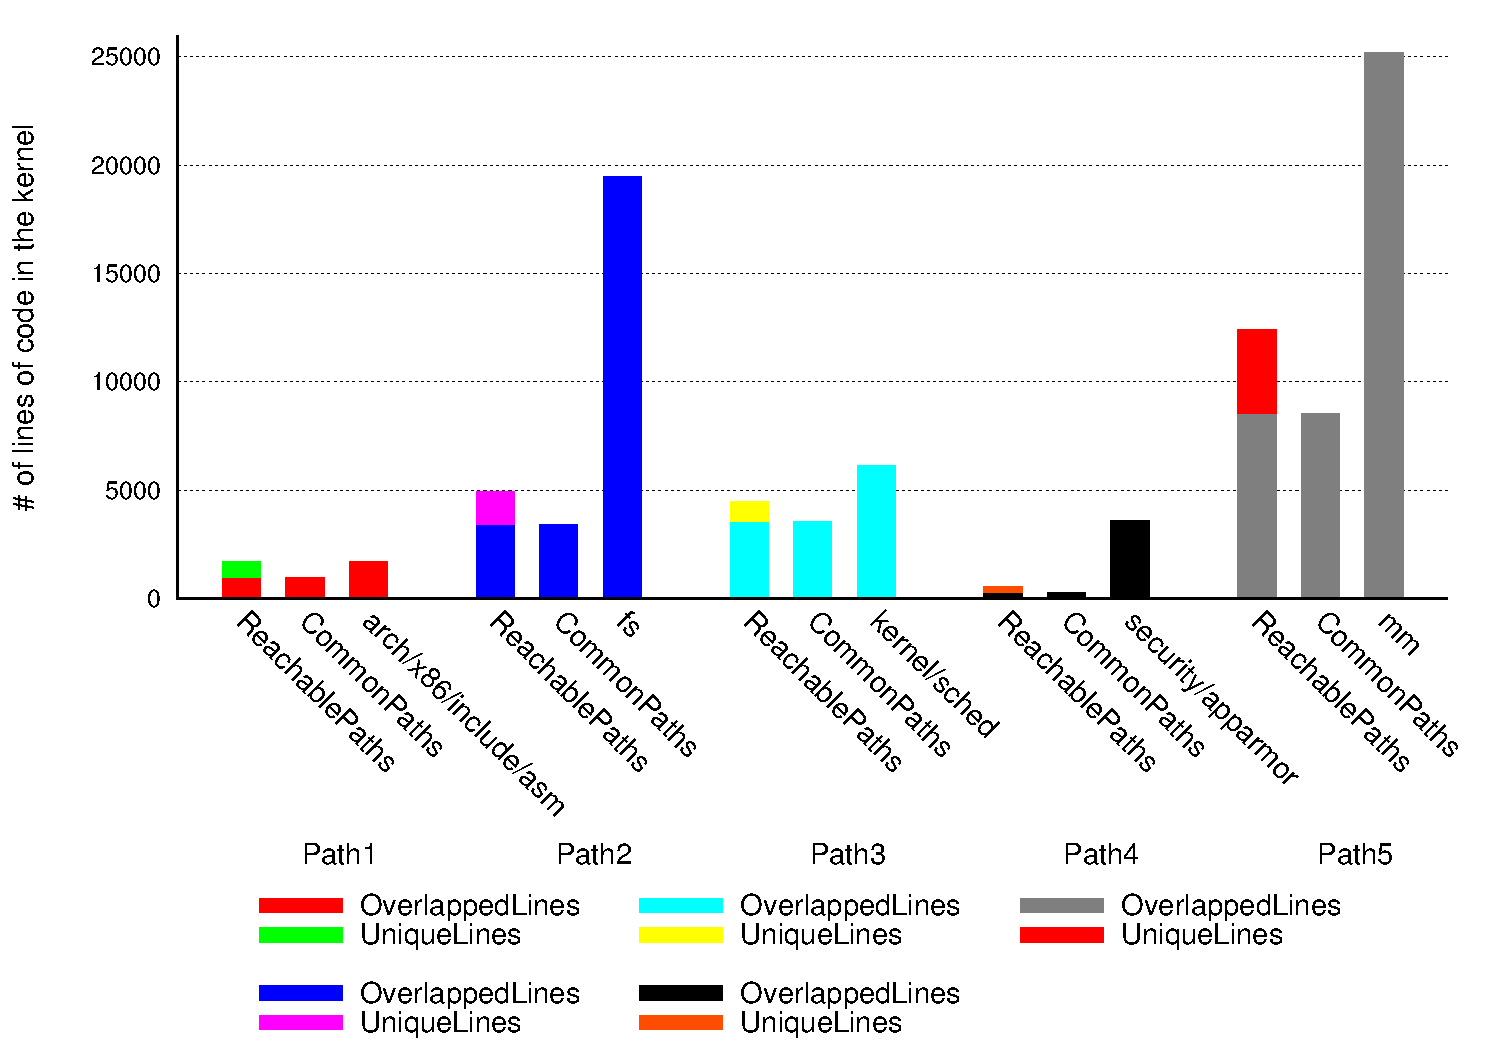
\includegraphics[width=1.0\columnwidth]{diagram/lind_oakland16_diagram_02.pdf}
\caption{Kernel Trace in Key Paths}
\label{fig:key_paths_trace}
\end{figure}

\subsubsection{Security Analysis of Kernel Paths\textendash Locating the
Risky Portions}

To verify our hypothesis, we next checked which portions of
the kernel contained kernel bugs. We examined 40 severe Linux kernel
bugs that had been discovered by the research community in the last five
years (the first two columns in Table 
\ref{table:vulnerabilities_commonly_used_kernel_paths}). 
We used these kernel bugs to check if vulnerabilities existed in certain
kernel traces.   \cappos{How?}
The results of our experiment are shown the last two columns in Table
\ref{table:vulnerabilities_commonly_used_kernel_paths}.

\begin{table*}[!ht]
\scriptsize
\centering
\begin{tabular}{|l|l|c|c|}\hline
\multirow{2}{*}{\textbf{Vulnerability}} & \multirow{2}{*}{\textbf{Specific
Type}} & \multicolumn{2}{c|}{\bf Portion of the Kernel} \\
\cline{3-4}
&  & \textbf{Total Reachable Paths} &  \textbf{Common Paths} \\ \hline

 CVE-2014-9529 & concurrency, race condition & {\color{red}\ding{51}} &
\ding{55} \\
 CVE-2014-3631 & NULL pointer dereference & {\color{red}\ding{51}} &
\ding{55} \\
 CVE-2012-6657 & network socket variable mischeck & {\color{red}\ding{51}}
& \ding{55} \\
 CVE-2014-5207 & privilege escalation & \ding{55} & \ding{55} \\
 CVE-2014-5206 & privilege escalation & \ding{55} & \ding{55} \\
 CVE-2014-3153 & privilege escalation & \ding{55} & \ding{55} \\
 CVE-2014-2851 & privilege escalation & \ding{55} & \ding{55} \\
 CVE-2014-2706 & race condition, DoS & {\color{red}\ding{51}} & \ding{55}
\\
 CVE-2014-0100 & race condition, DoS & {\color{red}\ding{51}} & \ding{55}
\\
 CVE-2014-0049 & buffer overflow & \ding{55} & \ding{55} \\
 CVE-2012-6638 & DoS & {\color{red}\ding{51}} & \ding{55} \\
 CVE-2014-0038 & privilege escalation & \ding{55} & \ding{55} \\
 CVE-2013-6368 & privilege escalation & \ding{55} & \ding{55} \\
 CVE-2013-4587 & index error, privilege escalation & \ding{55} & \ding{55}
\\
 CVE-2013-4563 & size/boundary check, DoS & {\color{red}\ding{51}} &
\ding{55} \\
 CVE-2013-4348 & value validation error & \ding{55} & \ding{55} \\
 CVE-2013-4300 & privilege escalation & {\color{red}\ding{51}} & \ding{55}
\\
 CVE-2013-1943 & privilege escalation & \ding{55} & \ding{55} \\
 CVE-2013-2094 & privilege escalation & {\color{red}\ding{51}} & \ding{55}
\\
 CVE-2013-3301 & NULL pointer dereference, DoS & {\color{red}\ding{51}} &
\ding{55} \\
 CVE-2013-1858 & privilege escalation & {\color{red}\ding{51}} & \ding{55}
\\
 CVE-2013-1797 & use-after-free & {\color{red}\ding{51}} & \ding{55} \\
 CVE-2013-1763 & privilege escalation, index error & \ding{55} & \ding{55}
\\
 CVE-2013-0310 & NULL pointer dereference & \ding{55} & \ding{55} \\
 CVE-2012-2136 & heap-based buffer overflow & \ding{55} & \ding{55} \\
 CVE-2012-2100 & lack of sanity check  & \ding{55} & \ding{55} \\
 CVE-2012-0028 & privilege escalation & {\color{red}\ding{51}} & \ding{55}
\\
 CVE-2011-2517 & privilege escalation, buffer overflow &
{\color{red}\ding{51}} & \ding{55} \\
 CVE-2012-2123 & privilege escalation  & {\color{red}\ding{51}} & \ding{55}
\\
 CVE-2012-1146 & NULL pointer dereference  & \ding{55} & \ding{55} \\
 CVE-2012-0207 & divide-by-zero error and panic & \ding{55} & \ding{55} \\
 CVE-2011-2525 & NULL pointer dereference  & {\color{red}\ding{51}} &
\ding{55} \\
 CVE-2011-1076 & NULL pointer dereference  & {\color{red}\ding{51}} &
\ding{55} \\
 CVE-2011-2184 & NULL pointer dereference, none initialization & \ding{55}
& \ding{55} \\
 CVE-2010-2478 & integer overflow & {\color{red}\ding{51}} & \ding{55} \\
 CVE-2010-2960 & NULL pointer dereference  & \ding{55} & \ding{55} \\
 CVE-2010-2492 & privilege escalation, buffer overflow & \ding{55} &
\ding{55} \\
 CVE-2010-2240 & stack overflow & {\color{red}\ding{51}} &
{\color{red}\ding{51}}\\
 CVE-2010-1188 & use-after-free & \ding{55} & \ding{55} \\
 CVE-2010-0437 & NULL pointer dereference  & {\color{red}\ding{51}} &
\ding{55} \\ \hline
 \multicolumn{2}{|c|}{\bf Percentage contains bugs} & {\bf $50\%$} & {\bf
$2.5\%$} \\ \hline
\end{tabular}
\caption {Linux Kernel Bugs, and Vulnerabilities in Different Portions of
the Kernel 
({\color{red}\ding{51}}: vulnerability in paths; \ding{55}: vulnerability
not in paths)}
\label{table:vulnerabilities_commonly_used_kernel_paths}
\end{table*}

From the results, we can see that commonly used kernel paths contain only
2.5\% of the bugs we had targeted. 
Since the total reachable kernel paths contain 50\% of the bugs we
examined, 
our results show that commonly used kernel paths clearly contain fewer bugs
than other portions of the kernel. 
\cappos{Why?}
Our hypothesis and findings provide insights and guidelines for new designs
of secure systems, 
which will be discussed in the next section. 
\cappos{Is this statistically significant?}





\section{A New Design for Building Secure Systems}
\label{sec.design}

This section discusses how to use the observation
 that ``commonly used kernel paths'' contain fewer bugs 
(\S{\ref{sec.metric}}) to build better security systems.
The key idea of our design is that all code \emph{including the complex part
of the operating system API} must have a very small TCB that accesses only 
commonly used kernel paths. 
Complex and dangerous system functions, which may access the risky portion of the kernel, 
are reimplemented by our own code within a sandbox. 
Therefore, any bugs or failures within the implementation of those complex system functions 
will be contained by the sandbox, and will not have the chance to reach 
and trigger risky portions of the kernel. Thus, we call it a ``safe-reimplementation'' design.

\begin{figure}[h]
\centering
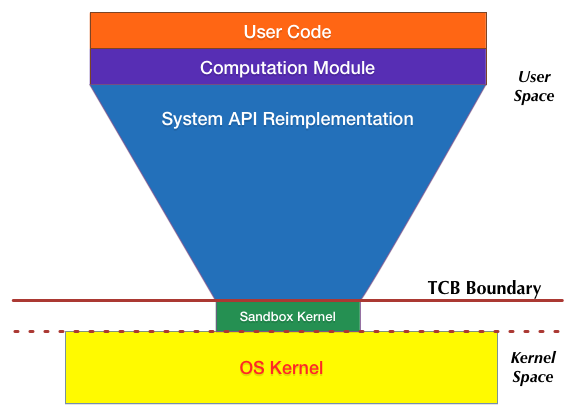
\includegraphics[width=1.0\columnwidth]{diagram/lind_secure_design.png}
\caption{The Idealized ``Safe-Reimplementation'' Design \cappos{This figure
needs to be edited I think.  The computation part doesn't fit...   Also,
perhaps there need to be ``bugs'' in the kernel, with most near the
outside parts.}}
\label{fig:design}
\end{figure}

\subsection{Architecture}

To execute untrusted applications in a safe manner that will not trigger bugs 
in the underlying OS kernel and cause damage to other parts of the system, 
our design intent is to build a sandbox system that can provide isolation and 
containment for any improper operations in the programs. 
One approach to building such a system is to place it entirely in the user space, 
and to only have a small sandbox kernel with restricted access to the OS kernel (Figure \ref{fig:design}). 
This approach has advantages over other approaches that require modifications to 
the OS kernel, because it avoids the risk of threat escalation. If modified modules 
are inside the OS kernel, they have kernel privileges that could allow attacks on the underlying OS, 
as well as applications run on top of it. 

There are two main components in our design of a secure sandbox system (Figure \ref{fig:design}). 
The first is a computation module, which performs functions like type checking, object creation, 
and garbage collection. The second is a system API that serves requests to access the OS kernel. 
Those two components should work together to complete the requirements of running user code. 
To run this code in our sandbox system, we first invoke the computation module to perform its operations. 
Whenever there are system call requests, 
the computation module will direct those requests to our system API. 
The system API will respond to the system call requests and return results to the user code if the requests are granted. 

\subsubsection{The Computation Module}

Our secure system should be able to support and run legacy applications, 
and execute binary code compiled from unmodified source code on popular hardware architecture, 
like x86 architecture. Providing an execution environment that can run unmodified source code is 
the main responsibility of the computation module. The key security issue of executing system calls 
without triggering OS kernel bugs is left to the system API module.

\subsubsection{The System API Module}

The system API module is the core of our sandbox system. It is comprised of two parts, 
a system API safe reimplementation, and the sandbox kernel. 

The sandbox kernel forms the only addition to the TCB of our system.  We 
make this system extremely small and simple so that it is easy to security
verify.  The purpose of the code is simply to provide an API that performs
a few critical system calls with the most basic parameters.  For example,
programs will need some mechanism to write data to the file system
and communicate with the network.  The kernel's goal is to provide the ability
to do so, while utilizing the most simplistic calls possible with the most
basic arguments.  For example, the file system API need only provide a way
to write data to storage.  It need not provide a directory abstraction, the
concept of file permissions, links, or even the concept of multiple files.
It merely needs to provide a mechanism to write out data that can be later
read in.  

%It should have a set of capabilities that enable the construction of essential and more complicated functions. 
%For example, the sandbox kernel capabilities should include basic functions for network, 
%file system I/O, lock, thread, and namespace. It also needs to have access to the OS kernel through system calls. 
%In developing our design, we leveraged our verified hypothesis that commonly used kernel paths contain fewer bugs. 
%Thus, the system calls we allow in our sandbox kernel are common calls, like file open, read, write, and close. 
%Furthermore, the set of arguments used for each call is also highly restricted. 

The system API safe reimplementation is a set of more complicated system calls 
that are constructed from our sandbox kernel. it should include reconstruction of 
complex system functions like many in the file system API. 
We reimplemented those system calls because we did not want user code 
to have direct access to the underlying OS kernel. 
Therefore, our reimplementation layer serves as a mediator between the user code 
and the OS kernel. In our design, the reimplementation is safe 
because the reconstruction of system calls is isolated in a sandbox. 
This can be done by choosing a memory-safe programming language to write code for the reimplementation. 
With this design, even if there are bugs in the function reimplementation, 
they cannot escape from the sandbox and will not reach the underlying OS kernel. 

Here is an example of how this reimplementation would work with the symbolic link function. 
\cappos{You likely need to talk about how you build this without the FS 
anyways.}  \cappos{Does a diagram showing the different design philosophies and
where they put functionality make sense?}
If there is a bug in this function, our safe reimplementation will not rely on the kernel code paths for symbolic links. 
Instead, our sandbox system will implement the (incorrect) buggy behavior, but do so within the sandbox. 
Since the reimplementation code does not have privileged access to the system as the OS kernel does, 
this will not result in a security issue. The usual outcome of a bug in this case is simply that the application will fail.

With the computation module and the system API module, unmodified user code is able to run on top of our designed system. 
It is important to note that our design does not rely on any specific technique or tool. 
To implement the computation module and the system API module in our design, 
it is possible to choose from several different techniques that fit well with the users' specific needs or requirements.

This general system design was implemented as a prototype secure system called Lind. 
In the next section, we provide a detailed description of Lind.

\section{Implementation of the Lind Prototype}
\label{sec.implementation}

Based on the design introduced in Section \S{\ref{sec.design}}, 
we implemented a secure sandbox system, Lind, 
for running untrusted user programs on vulnerable OS kernels. 
Lind adapts two basic  technologies as its building blocks\textendash Google's Native Client, and Seattle's Repy. 
As described in \S{\ref{sec.design}} (Figure \ref{fig:design}), our design has  two main components\textendash a computation module 
and a system API module. Google's Native Client served as the computation module 
and Seattle's Repy as the system API module (Figure \ref{fig:architecture}).

\begin{figure}[h]
\centering
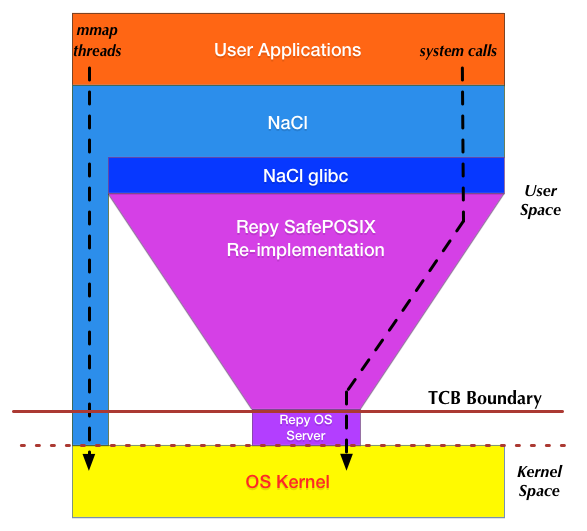
\includegraphics[width=1.0\columnwidth]{diagram/lind_architecture.png}
\caption{System Overview of Lind}
\label{fig:architecture}
\end{figure}

\subsection{The Computation Module of Lind: Google's Native Client}
We use Google's Native Client (NaCl) \cite{NaCl-09} as our computation module 
because it provides an environment for efficient execution of legacy code in the form of x86 and ARM binaries. 
NaCl can perform the functions required by the computation module well, and it is easy to 
connect with our system API module because NaCl uses glibc to perform system calls. 
Modification to NaCl's glibc would allow us to redirect those system call requests to our own system API module. 

NaCl is a sandbox used to execute untrusted x86 native code. 
It aims to give applications the computational performance of native applications without compromising safety. 
NaCl uses software fault isolation and a secure runtime to direct system interaction and 
side effects through interfaces managed by the program. It provides operating system portability 
for binary code while supporting performance-oriented features, such as thread support, 
instruction set extensions, such as SSE, and use of compiler intrinsics and a hand-coded assembler. 
It also allows the efficient execution of legacy code in the form of x86 and ARM binaries 
that are built with a lightly modified compiler tool chain. 

\subsection{The System API Module of Lind: Seattle's Repy}

Seattle's Repy \cite{Repy-10} is a restricted subset of Python, that works as a sandbox to provide a safer environment 
to run applications. For Lind, we used Repy to build our system API module. 
To be more specific, our system API module has a very small sandbox kernel as TCB,  
written with Python. On top of the sandbox kernel, 
we use Repy code to safely reimplement complex system functions.

\subsubsection{The Repy Sandbox Kernel}

As we have discussed in \S{\ref{sec.design}}, the sandbox kernel needs to be secure and bug-free. 
Because it is the TCB of the system, any bugs within it could cause fatal problems, 
and allow attackers to access the OS kernel and gain kernel privilege. 
Seattle's Repy was selected as our system API module, because it has a very small sandbox kernel, 
comprised of only 8K LOC. Using Repy also demonstrated our key design principle that 
our system should only access the safe portions of the OS kernel. In the Repy sandbox kernel, 
there are 33 basic API functions, including 13 network functions, 6 file functions, 6 threading functions, 
and 8 miscellaneous functions (Table \ref{table:RepyKernel}) \cite{Repy-10}, \cite{RepyKernel}. Most of those functions are simple and 
regularly used system calls that access the commonly used kernel paths. 

\begin{table}
\centering
\scriptsize
\begin{tabular}{|c|l|}
  \hline
  \textbf{Network Functions} & \textbf{API Function Name} \\
  \hline
  01 & gethostbyname(name) \\
  \hline
  02 & getmyip() \\
  \hline
  03 & sendmessage(destip, destport, message, localip, localport) \\
  \hline
  04 & openconnection(destip, destport, localip, localport, timeout) \\
  \hline
  05 & socket.close() \\
  \hline
  06 & socket.recv(numbytes) \\
  \hline
  07 & socket.send(message) \\
  \hline
  08 & listenforconnection(localip, localport) \\
  \hline
  09 & tcpserversocket.getconnection() \\
  \hline
  10 & tcpserversocket.close()\\
  \hline
  11 & listenformessage(localip, localport) \\
  \hline
  12 & udpserversocket.getmessage() \\
  \hline
  13 & udpserversocket.close() \\
  \hline \hline
  \textbf{File Functions} & \textbf{API Function Name} \\
  \hline
  01 & openfile(filename, create) \\
  \hline
  02 & file.close() \\
  \hline
  03 & file.readat(sizelimit, offset) \\
  \hline
  04 & file.writeat(data, offset) \\
  \hline
  05 & listfiles() \\
  \hline
  06 & removefile(filename) \\
  \hline \hline
  \textbf{Threading Functions} & \textbf{API Function Name} \\
  \hline
  01 & createlock() \\
  \hline
  02 & lock.acquire(blocking) \\
  \hline
  03 & lock.release() \\
  \hline
  04 & createthread(function) \\
  \hline
  05 & sleep(seconds) \\
  \hline
  06 & getthreadname() \\
  \hline \hline
  \textbf{Miscellaneous Functions} & \textbf{API Function Name} \\
  \hline
  01 & log(*args) \\
  \hline
  02 & getruntime() \\
  \hline
  03 & randombytes() \\
  \hline
  04 & exitall() \\
  \hline
  05 & createvirtualnamespace(code, name) \\
  \hline
  06 & virtualnamespace.evaluate(context) \\
  \hline
  07 & getresources() \\
  \hline
  08 & getlasterror() \\
  \hline
\end{tabular}
\caption {System Functions in the Repy Sandbox Kernel}
\label{table:RepyKernel}
\end{table}

\subsubsection{The SafePOSIX Reimplementation}

The key responsibility of our system API module is to serve system call requests from user code. 
In the Lind system, those system call requests are issued from the user code, 
received by the computation module NaCl, and then redirected to our system API module. 
The API module includes a POSIX API to serve those requests. 

A POSIX API is a set of standard operating system interfaces that provide operating system functions 
to the user code. However, the POSIX API is large and complex, which means 
it would be really difficult to ensure that its implementation is secure and bug-free. 
Our choice to use Repy helped us solve this key security problem. 
Since Repy is a programming language sandbox, it can provide the ideal isolation 
we needed when constructing our POSIX API. In Lind, 
complex system functions are reimplemented using Repy code, 
based on the ``safe-reimplement'' principle from our design in \S{\ref{sec.design}}.

\subsection{Operations}

Here, we take a closer look at how Lind functions when an application seeks access. 
This discussion focuses mainly on the connection between Google's Native Client and Seattle's Repy sandbox.

Lind combines the NaCl and Repy component to provide native computation and 
safe access to the system. Untrusted programs are run in NaCl, 
but access to all system resources is diverted to a Repy program. 
This program is responsible for accessing the system on behalf of the program, 
which is called the Lind library OS. A NaCl sandbox is built on top of the Repy sandbox. 
To service a system call in NaCl, a server routine marshals its arguments into a text string, 
and sends the call and the arguments to Repy sandbox. 
The library OS then executes the appropriate system call, marshals the result and 
returns it back to NaCl. The result is eventually returned as the appropriate native type to the calling program. 

Lind is designed to minimize its modifications within the TCB of these two sandboxes. 
By running the Lind code is run from within the two sandboxes, 
the modifications to the sandboxes themselves (and therefore the TCB) were extremely small. 

The only complex part of Lind is the library OS, which runs in Repy. 
However, because Python is a very powerful language that provide rich functions, 
it significantly simplified the construction of Lind. Even though Python is considered ``slow'' by some, 
the internals of an application in Lind are run in NaCl, a very high performance environment. 
This balances the performance of the system, with the ease of implementation and maintenance 
of the library OS component of Lind. 

Furthermore, this particular design and architecture for sandboxing ensures the programs are portable. 
Programs running inside Lind are written to work against a standard POSIX glibc interface, 
and, since the Lind runtime is strictly user-level, it can work on many different platforms 
including Linux, Mac OS X and Windows.

Finally, Lind is lightweight. Because the sandbox only incurs overhead when there is a system call, 
overall overhead for Lind is low. Lind uses a native interface for execution, 
allowing CPU-and-memory-intensive applications to run at speeds that are equivalent to NaCl and near native speed. 

\subsection{The Benefits of the Two Sandbox System}

In reviewing the design of Lind, some fundamental questions could be raised about the dual sandbox design. 
Why is one not enough? And, if two is good, why not use more? 
The answer to the first question is that the kernel interface is extremely rich and hard to protect. 
In order to have minimal impact on the kernel, as well as provide sufficient API for legacy applications, 
we need to have one sandbox focuses on protecting the kernel and providing POSIX API, 
while a second sandbox focuses on efficiently executing applications. 
So our approach includes two sandboxes, one as the computation module, 
and the other one as system API module. As to the second question, 
which could be rephrased as ``why not sandbox Repy TCB and get more security?,'' 
the lowest level sandbox eventually must have some fundamental, 
even if  limited access to system resources, such as memory, and storage, threads. 
So even if we were to sandbox Repy TCB and have additional sandboxes, 
the one at the bottom level will still access the OS kernel in a similar way. 
Thus, having multiple sandboxes does not provide any extra security benefits. 

In \S{\ref{sec.evaluation}}, we present how the dual sandboxes and other elements of Lind performed in 
head-to-head evaluation against other virtualization systems.
\section{Evaluation}
\label{sec.evaluation}

In seeking to evaluate the performance of Lind, 
we designed and conducted a set of experiments based around four
fundamental 
questions:

\begin{itemize}
\item What are the benefits of running applications in Lind, 
and not in other existing virtualization systems?
(\S{\ref{Linux-Kernel-Bug-Test-and-Evaluation}})

\item Why is Lind less likely to trigger kernel bugs compared to 
other virtualization systems?
(\S{\ref{Reachable-Kernel-Trace-Analysis-for-Different-Virtualization-Systems}})

\item Is Lind really secure? What happens if one of the building blocks
of Lind, 
the Repy sandbox kernel has bugs?
(\S{\ref{Reachable-Kernel-Trace-Analysis-for-Repy-Sandbox}})

\item Is Lind a practical tool that can run real-world applications at
reasonable overhead? 
(\S{\ref{Performance-Evaluation}})
\end{itemize}

In this section, we describe the experiments designed to answer these
question, 
and discuss how the results support the merits of our secure design and its
prototype Lind. 

\subsection{Evaluation Methodology}

Our evaluation strategy was to directly compare the performance of Lind
against 
four other existing virtualization systems\textendash VirtualBox, VMWare
Workstation, 
Docker, and Graphene. We also compared it against Native Linux and used 
those results as a baseline for evaluation. Because Native Linux is the
original OS, 
without virtualization and additional protection, this data helps to
clarify the security benefits of Lind, 
as well as whatever performance overhead costs the system may incur.

\textbf{Experimental setup.}
We conducted our experiments under Linux kernel 3.14.1, using the following
protocols:

\begin{itemize}
\item We identified and examined a list of  69 historical bugs that have
specifically 
targeted Linux kernel 3.14.1 \cite{CVE-Datasource}. Through analyzing
security kernel patches for those bugs, 
we identified the lines of code in the kernel that correspond to each of
one.

\item In order to test if a bug is triggerable, we created or located C
code to 
exploit each of the kernel bugs \cite{Exploit-Database}. We were able to
run and obtain results for 
35 out of the 69 bugs in our experiments. For the rest of the bugs, 
we could not find exploit code that would trigger them effectively at that
moment. 
In addition, it was very difficult to accurately determine if more complex
bugs 
were triggered or not. We leave further study and analysis of those bugs to
future work.

\item We compiled and ran the exploit C code under each virtualization
system to 
obtain their kernel traces, and then used our kernel trace safety metric to
determine 
if a specific bug was triggered inside that virtualization system. 

\item Lastly, to  analyze the reachable kernel paths for each of the
virtualization systems, 
we conducted system call fuzzing (similar to what we did in ?3) to obtain
the kernel trace in each system. 
We repeated the system call fuzzing within Repy as well to obtain its
kernel trace. 
\end{itemize}

\subsection{Comparison Results and Analysis}

Since our primary goal was to build a secure system, our core evaluation
was conducted primarily 
from a security perspective
(\S{\ref{Linux-Kernel-Bug-Test-and-Evaluation}}, 
\S{\ref{Reachable-Kernel-Trace-Analysis-for-Different-Virtualization-Systems}}, 
\S{\ref{Reachable-Kernel-Trace-Analysis-for-Repy-Sandbox}}). 
We also conducted an evaluation of the performance overhead of Lind
(\S{\ref{Performance-Evaluation}}) 
to obtain some understanding of its potential overall efficacy in
real-world settings.

\subsubsection{Linux Kernel Bug Test and Evaluation}
\label{Linux-Kernel-Bug-Test-and-Evaluation}

We tested 35 Linux kernel bugs in Native Linux, VirtualBox, VMWare
Workstation, Docker, Graphene, 
and Lind, to evaluate if any of them can be triggered. The kernel bugs
examined 
are capable of causing serious security problems. For example, 
the CVE-2014-8989 bug allows local users to bypass intended file
permissions by leveraging a POSIX ACL. 
When running applications, the potential risk of triggering some of these
kernel bugs here, 
and possibly many more bugs outside our list, is a severe problem that
users should be concerned about.

The results of verifying which kernel bugs were triggered under each
environment is illustrated in Table \ref{table:trigger_vulnerabilities}. 
We found that a substantial number of bugs were triggered in existing
virtualization systems. 
A full 35 out of 35 (100\%) bugs were triggered in Native Linux, 
while the other programs had somewhat lower rates: 14/35 (40\%) in
VirtualBox, 
11/35 (31.4\%)  in VMWare Workstation, 8/35 (22.9\%)  in Docker, and 8/35
(22.9\%) bugs in Graphene. 
In comparison, only 1 out of 35 bugs  (2.9\%)  was triggered in Lind. 
Comparing these results, Lind worked significantly better than the other
systems in limiting the triggering of kernel bugs.

\begin{table*}[!ht]
\scriptsize
\centering
\caption {Linux Kernel Bugs, and Vulnerabilities in Different
Virtualization Systems 
({\color{red}\ding{51}}: vulnerability triggered; \ding{55}: vulnerability
not triggered)}
\begin{tabular}{|l|c|c|c|c|c|c|}\hline
\textbf{Vulnerability}    &  \textbf{Native Linux}  &  \textbf{VirtualBox}
&  \textbf{VMWare Workstation}
 & \textbf{Docker} & \textbf{Graphene} & \textbf{Lind} \\
\hline
 CVE-2015-5706 & {\color{red}\ding{51}} & {\color{red}\ding{51}} &
{\color{red}\ding{51}} & {\color{red}\ding{51}} & {\color{red}\ding{51}} &
\ding{55}  \\
 CVE-2015-0239 & {\color{red}\ding{51}} & {\color{red}\ding{51}} &
{\color{red}\ding{51}} & \ding{55} & \ding{55}  & \ding{55}  \\
 CVE-2014-9584 & {\color{red}\ding{51}} & \ding{55}  & \ding{55}  &
\ding{55} & \ding{55}  & \ding{55}  \\
 CVE-2014-9529 & {\color{red}\ding{51}} & {\color{red}\ding{51}}  &
\ding{55}  & \ding{55} & \ding{55}  & \ding{55}  \\
 CVE-2014-9322 & {\color{red}\ding{51}} & {\color{red}\ding{51}}  &
\ding{55}  & {\color{red}\ding{51}} & {\color{red}\ding{51}}  & \ding{55}
\\
 CVE-2014-9090 & {\color{red}\ding{51}} & \ding{55}  & \ding{55}  &
\ding{55} & \ding{55}  & \ding{55}  \\
 CVE-2014-8989 & {\color{red}\ding{51}} & {\color{red}\ding{51}} &
{\color{red}\ding{51}} & {\color{red}\ding{51}} & {\color{red}\ding{51}} &
\ding{55}  \\
 CVE-2014-8559 & {\color{red}\ding{51}} & \ding{55}  & \ding{55}  &
\ding{55} & \ding{55}  & \ding{55}  \\
 CVE-2014-8369 & {\color{red}\ding{51}} & \ding{55}  & \ding{55}  &
\ding{55} & \ding{55}  & \ding{55}  \\
 CVE-2014-8160 & {\color{red}\ding{51}} & {\color{red}\ding{51}} &
{\color{red}\ding{51}} & \ding{55} & \ding{55}  & \ding{55}  \\
 CVE-2014-8134 & {\color{red}\ding{51}} & {\color{red}\ding{51}} &
{\color{red}\ding{51}} & \ding{55} & {\color{red}\ding{51}}  & \ding{55}
\\
 CVE-2014-8133 & {\color{red}\ding{51}} & {\color{red}\ding{51}}  &
\ding{55}  & \ding{55} & \ding{55}  & \ding{55}  \\
 CVE-2014-8086 & {\color{red}\ding{51}} & {\color{red}\ding{51}} &
{\color{red}\ding{51}} & {\color{red}\ding{51}} & \ding{55} & \ding{55}  \\
 CVE-2014-7975 & {\color{red}\ding{51}} & \ding{55}  & \ding{55}  &
\ding{55} & \ding{55}  & \ding{55}  \\
 CVE-2014-7970 & {\color{red}\ding{51}} & \ding{55}  & \ding{55}  &
\ding{55} & \ding{55}  & \ding{55}  \\
 CVE-2014-7842 & {\color{red}\ding{51}} & \ding{55}  & \ding{55}  &
\ding{55} & \ding{55}  & \ding{55}  \\
 CVE-2014-7826 & {\color{red}\ding{51}} & {\color{red}\ding{51}} &
{\color{red}\ding{51}} & \ding{55} & {\color{red}\ding{51}}  & \ding{55}
\\
 CVE-2014-7825 & {\color{red}\ding{51}} & {\color{red}\ding{51}} &
{\color{red}\ding{51}} & \ding{55} & {\color{red}\ding{51}}  & \ding{55}
\\
 CVE-2014-7283 & {\color{red}\ding{51}} & \ding{55}  & \ding{55}  &
\ding{55} & \ding{55}  & \ding{55}  \\
 CVE-2014-5207 & {\color{red}\ding{51}} & \ding{55}  & \ding{55}  &
\ding{55} & \ding{55}  & \ding{55}  \\
 CVE-2014-5206 & {\color{red}\ding{51}} & \ding{55}  &
{\color{red}\ding{51}}  & {\color{red}\ding{51}}& \ding{55}  & \ding{55}
\\
 CVE-2014-5045 & {\color{red}\ding{51}} & \ding{55}  & \ding{55}  &
\ding{55} & \ding{55}  & \ding{55}  \\
 CVE-2014-4943 & {\color{red}\ding{51}} & \ding{55}  & \ding{55}  &
\ding{55} & \ding{55}  & \ding{55}  \\
 CVE-2014-4667 & {\color{red}\ding{51}} & \ding{55}  & \ding{55}  &
\ding{55} & {\color{red}\ding{51}}  & \ding{55}  \\
 CVE-2014-4508 & {\color{red}\ding{51}} & \ding{55}  & \ding{55}  &
\ding{55} & \ding{55}  & \ding{55}  \\
 CVE-2014-4171 & {\color{red}\ding{51}} & {\color{red}\ding{51}} &
{\color{red}\ding{51}} & {\color{red}\ding{51}} & {\color{red}\ding{51}} &
{\color{red}\ding{51}}  \\
 CVE-2014-4157 & {\color{red}\ding{51}} & \ding{55}  & \ding{55}  &
\ding{55} & \ding{55}  & \ding{55}  \\
 CVE-2014-4014 & {\color{red}\ding{51}} & \ding{55}  &
{\color{red}\ding{51}}  & {\color{red}\ding{51}} & \ding{55}  & \ding{55}
\\
 CVE-2014-3940 & {\color{red}\ding{51}} & {\color{red}\ding{51}}  &
\ding{55}  & {\color{red}\ding{51}}& \ding{55}  & \ding{55}  \\
 CVE-2014-3917 & {\color{red}\ding{51}} & {\color{red}\ding{51}}  &
\ding{55}  & \ding{55} & \ding{55}  & \ding{55}  \\
 CVE-2014-3153 & {\color{red}\ding{51}} & \ding{55}  & \ding{55}  &
\ding{55} & \ding{55}  & \ding{55}  \\
 CVE-2014-3144 & {\color{red}\ding{51}} & \ding{55}  & \ding{55}  &
\ding{55} & \ding{55}  & \ding{55}  \\
 CVE-2014-3122 & {\color{red}\ding{51}} & \ding{55}  & \ding{55}  &
\ding{55} & \ding{55}  & \ding{55}  \\
 CVE-2014-2851 & {\color{red}\ding{51}} & \ding{55}  & \ding{55}  &
\ding{55} & \ding{55}  & \ding{55}  \\
 CVE-2014-0206 & {\color{red}\ding{51}} & \ding{55}  & \ding{55}  &
\ding{55} & \ding{55}  & \ding{55}  \\
\hline
\end{tabular}
\label{table:trigger_vulnerabilities}
\end{table*}

\subsubsection{Reachable Kernel Trace Analysis for Different Virtualization
Systems}
\label{Reachable-Kernel-Trace-Analysis-for-Different-Virtualization-Systems}

After establishing that Lind was efficient at finding bugs, our next step
was to examine how Lind was able to achieve this efficiency.  
To answer this question, we obtained the total reachable kernel trace for
each of the systems (including Lind) 
and did further analysis on the components of those traces. These results
are listed in Table \ref{table:trace-systems}.

As the numbers reveal, Lind accessed the minimum amount of code in the OS
kernel. More importantly, 
all the kernel code it accessed was in the safe portion of the kernel, the
commonly used kernel paths. 
As we have already verified in ?3.3\cappos{make link}, the safe portion of 
the kernel contains fewer kernel bugs. 
So it make sense that Lind is less likely to trigger kernel bugs. 

The other virtualization systems all accessed a substantial number of code
paths in the kernel, 
and they all had access to a larger section of the risky portion, the
uncommonly used kernel paths. 
Based on our hypothesis, many historical bugs, as well as undetected
zero-day bugs, could be located there. 
Thus, accessing the risky portion without restriction is dangerous, and
leads to kernel bug exploitation. 

To summarize, the secret of how Lind is able to trigger the least kernel
bugs lies in the important fact that 
it is better able to control access to the OS kernel. 
Thus, we would assert the better results achieved with Lind is a natural
outcome of its design.

\begin{table}
\centering
\scriptsize
\caption{Reachable Kernel Trace Analysis for Different Virtualization
Systems}
\begin{tabular}{|l|l|l|l|}
  \hline
  \multirow{3}{1.5cm}{\bf Virtualization system} & \multicolumn{3}{c|}{\bf Kernel trace} \\ \cline{2-4}
  & \multirow{2}{1.5cm}{Compared to native Linux} & \multirow{2}{1.8cm}{In safe portion 
  (common paths)} & \multirow{2}{2cm}{In risky portion (uncommon paths)} \\
  & & & \\  \hline
  VirtualBox & 78.8 \% & 46.5 \% & 53.5 \% \\
  \hline
  \multirow{2}{1.5cm}{VMWare Workstation} & \multirow{2}{*}{72.6 \%} & 
  \multirow{2}{*}{50.2 \%} & \multirow{2}{*}{49.8 \%} \\ 
  & & & \\   \hline
  Docker & 61.3 \% & 58.4 \% & 41.6 \% \\
  \hline
  Graphene & 49.2 \% & 65.1 \% & 34.9 \% \\
  \hline
  Lind & 36.2 \% & 100 \% & 0 \% \\
  \hline
\end{tabular}
\label{table:trace-systems}
\end{table}

\subsubsection{Reachable Kernel Trace Analysis for Repy Sandbox}
\label{Reachable-Kernel-Trace-Analysis-for-Repy-Sandbox}

An important question about Lind's security guarantee is what happens if
there is a bug or a failure in Lind's TCB, 
the Repy sandbox kernel. Because the TCB has direct access to the OS
kernel, if a bug occurs in the TCB, 
it can potentially access the privileged OS kernel and trigger kernel bugs. 

To determine if a flaw in the TCB could endanger a kernel, 
we obtained the total reachable kernel trace in Repy and analyzed its
components. 
The results are shown in Table \ref{table:trace-Repy}. The trace of Repy is
slightly larger (5.8\%) than that of Lind, 
which means that Repy's design can not allow attackers or bugs to 
have much access to the OS kernel. In fact, only a small amount (5.8\%) of
additional OS kernel paths might be open. 
More importantly, The kernel trace of Repy lies completely within the safe
portion of the OS kernel. 
Since the safe portion contains fewer kernel bugs, the Repy sandbox kernel
will have a very slim chance to trigger OS kernel bugs.

The design explained above shows that even if our Repy sandbox kernel has a
bug or failure inside, 
it only slightly increases the amount of OS kernel paths open to attacks,
and all these paths accessed are still inside the safe portion. 
Therefore, Repy will not grant attackers more opportunities to trigger OS
kernel bugs. 
Since Repy, arguably the main security weakness of the system, can be
considered safe by our analysis, 
it shows that Lind can provide strong security to run user applications.

\begin{table}
\centering
\scriptsize
\caption{Reachable Kernel Trace Analysis for the Repy Sandbox.  \cappos{Is
this correct?}}
\begin{tabular}{|l|l|l|l|l|}
  \hline
  \multirow{3}{.8cm}{\bf Sandbox} & \multicolumn{4}{c|}{\bf Kernel trace} \\ \cline{2-5}
  & \multirow{2}{1cm}{Compared to Lind} & 
  \multirow{2}{1.3cm}{Compared to native Linux} & \multirow{2}{1.7cm}{In safe portion 
  (common paths)} & \multirow{2}{1.9cm}{In risky portion (uncommon paths)} \\
  & & & & \\  \hline
  
%  Sandbox &  \thead{Kernel Trace \\ Compared to \\ Lind} & \thead{Kernel
%Trace \\ Compared to \\ Native Linux} &
%  \thead{Kernel Trace \\ in Safe Portion \\ (Common Paths)} & \thead{Kernel
%Trace \\ in Risky Portion \\ (Uncommon Paths)} \\
%  \hline
  Repy & 105.8 \% & 38.3 \% & 100 \%  & 0 \%  \\
  \hline
\end{tabular}
\label{table:trace-Repy}
\end{table}

\subsubsection{Performance Evaluation}
\label{Performance-Evaluation}

Since security systems still need to be efficient, economically and in
terms of performance, 
we also set up a test to demonstrate that Lind is a practical tool. 
We ran a variety of real-world applications in Lind and compared runtime
performance 
against that in Native Linux to measure the overhead cost it could incur.

We first compiled and ran three widely used applications, 
a primes calculator, GNU grep, and GNU wget. All ran unaltered and
correctly inside Lind. The source code of each of the applications remains 
unmodified. To run them, it is sufficient to just recompile the source code with 
NaCl's GNU tool chain.
Figure \ref{fig:performance_applications} shows the runtime performance
results. 
The primes application ran in Lind has a 6\% performance overhead compared to 
Native Linux. CPU bound applications, like the primes, generally experience small overhead, 
because they run only inside the NaCl computation sandbox. No system calls are required, 
and there is no need to go through the safe POSIX interface. The small amount of overhead 
is generated by NaCl's instruction alignment at the building time. Another reason for the overhead 
is that the instructions built by NaCl have a higher rate of cache misses, which can slowdown the 
program. 
We expect other CPU bound processes to behave similarly. 
Grep experienced roughly 11x slowdown over Native Linux, while the Wget
slowdown was roughly 19x. Since they are both system-call heavy applications, they need to go 
through our safe POSIX interface to access the kernel, which produced the overhead.  

\begin{figure}
\centering
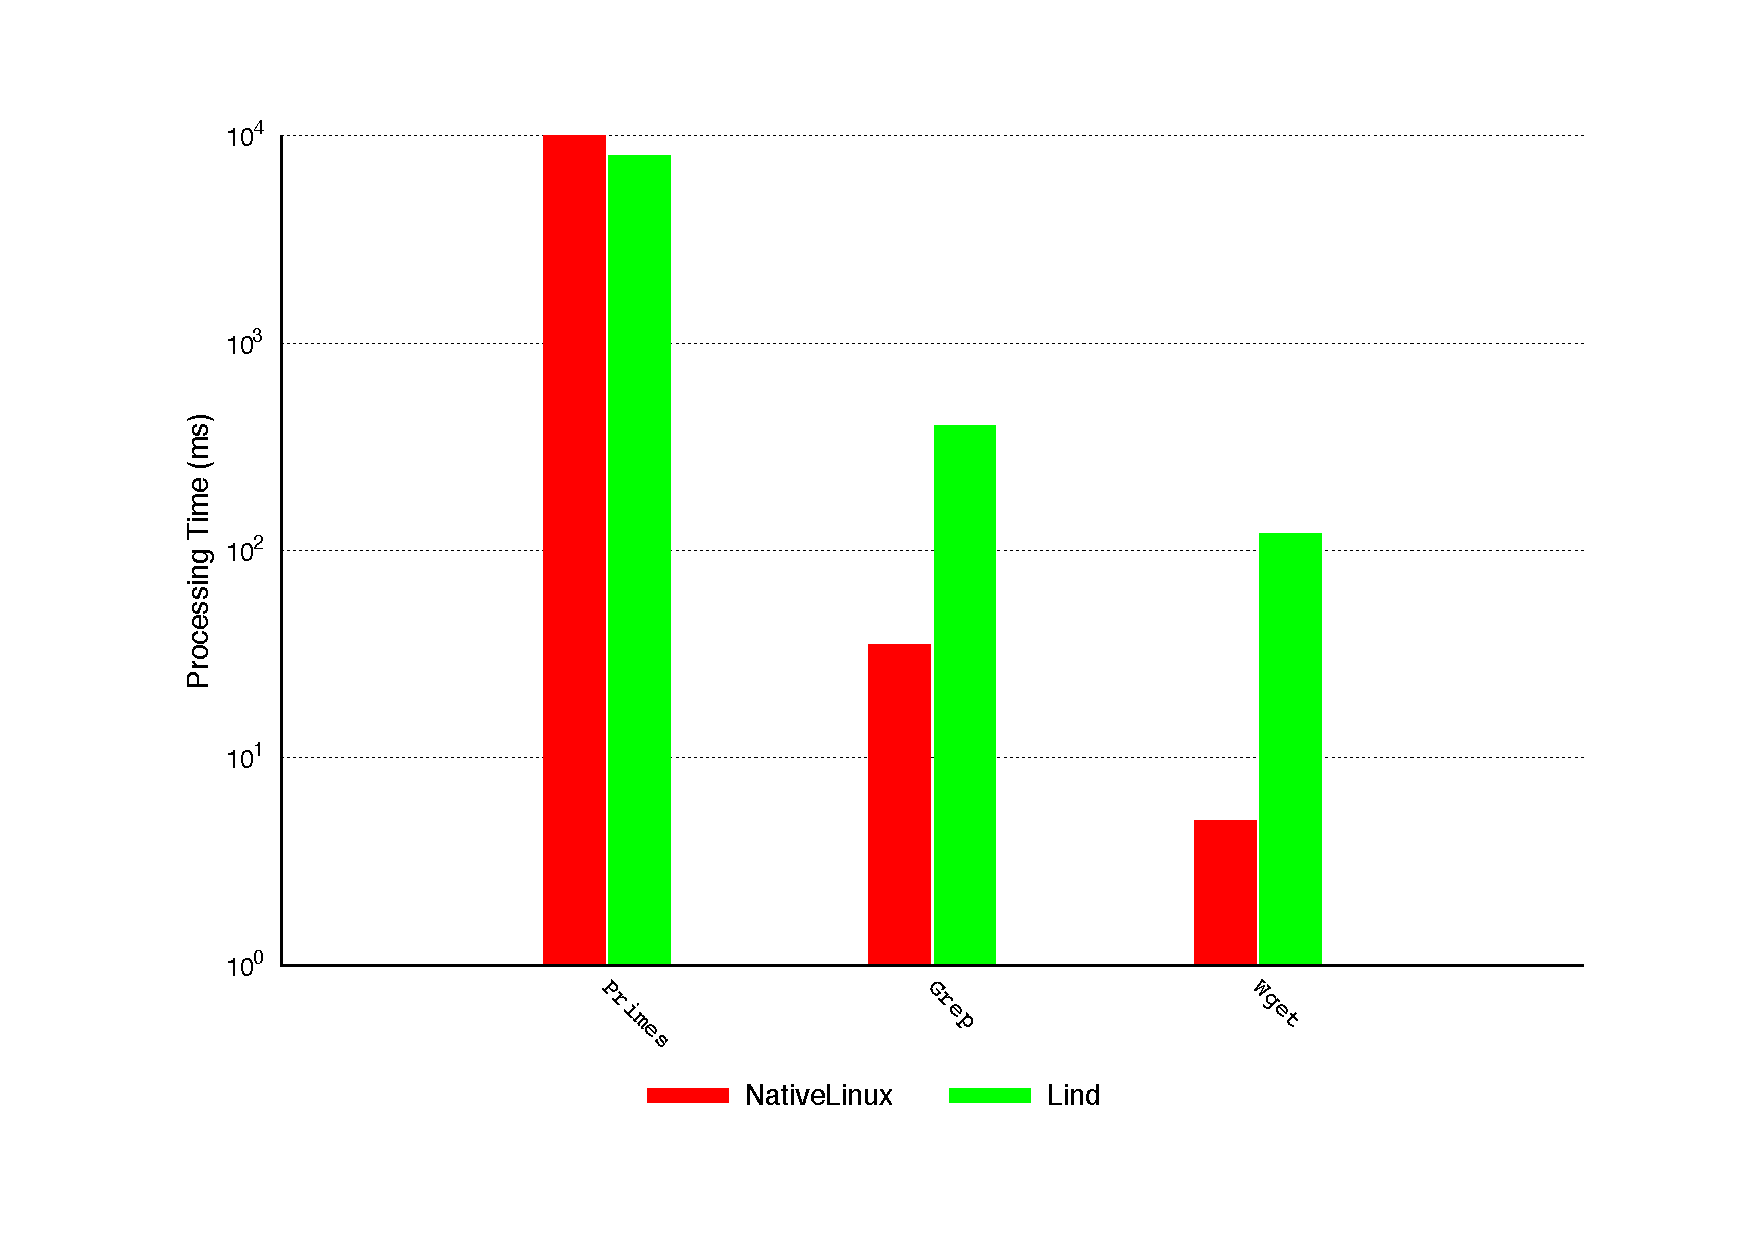
\includegraphics[width=1.0\columnwidth]{diagram/lind_oakland16_performance.pdf}
\caption{Applications Runtime Performance: Native Linux vs. Lind}
\label{fig:performance_applications}
\end{figure}

Next, we ran the legacy application Tor in Lind. Tor runs unmodified in
Lind. We used NaCl's gcc compiler to build the binary that could run in NaCl. 
We used the benchmarks that come with Tor to test several of its common
operations. 
A summary of the results is shown in Table \ref{table:performance_tor}. The
benchmarks focus on cryptographic operations, 
which are CPU intensive, but also make system calls like getpid, and reads to
/dev/urandom.
The digest operations time the access of a map of message digests. 
The AES operations time AES encryptions of several sizes and message 
digest creation. 
Cell processing executes full packet encryption and decryption. In our
test, 
Lind slowed these operations between 2.5x and 5x. We believe these
slowdowns 
are caused by the increased code size produced by NaCl, and the
increased overhead from Lind's safe POSIX system call interface. 

As shown above,  Lind does incur some performance overhead in most cases. 
It should be noted though that, at this point, we have not  yet attempted
to optimize its performance. 
It might be argued that, since an attack on the kernel can have devastating
result, at this initial stage, 
a tradeoff between security and performance is justified. Despite this
issue, 
the fact that Lind is able to run many legacy applications suggests that it
is a positive step towards building new secure systems. 

\begin{table}
\centering
\scriptsize
\caption{Performance Results on Tor's Built-in Benchmark Program: Native
Linux vs. Lind.}
\begin{tabular}{|r|r|r|r|}
  \hline
  Benchmark & Native Code & Lind & Impact  \\
  \hline
  Digest Tests: & & & \\
  Set & 54.80 nsec/element & 176.86 nsec/element & 3.22x \\
  Get & 42.30 nsec/element & 134.38 nsec/element & 3.17x \\
  Add & 11.69 nsec/element & 53.91 nsec/element & 4.61x \\
  IsIn & 8.24 nsec/element & 39.82 nsec/element & 4.83x \\
  \hline
  AES Tests: & & & \\
  1 Byte & 14.83 nsec/B & 36.93 nsec/B & 2.49x \\
  16 Byte & 7.45 nsec/B & 16.95 nsec/B & 2.28x \\
  1024 Byte & 6.91 nsec/B & 15.42 nsec/B & 2.23x \\
  4096 Byte & 6.96 nsec/B & 15.35 nsec/B & 2.21x \\
  8192 Byte & 6.94 nsec/B & 15.47 nsec/B & 2.23x \\
  Cell Sized & 6.81 nsec/B & 14.71 nsec/B & 2.16x \\
  \hline
  Cell Processing: & & & \\
  Inbound & 3378.18 nsec/cell & 8418.03 nsec/cell & 2.49x \\
  (per Byte) & 6.64 nsec/B & 16.54 nsec/B & - \\
  Outbound & 3384.01 nsec/cell & 8127.42 nsec/cell & 2.40x \\
  (per Byte) & 6.65 nsec/B & 15.97 nsec/B & - \\
  \hline
\end{tabular}
\label{table:performance_tor}
\end{table}


\section{Study Limitations/Exceptions and Future Work}
\label{sec.limitation}


While these early results are promising, it should be noted that there were
a few limitations on the scope of the study that may need to be addressed
in future studies. First of all, our metric relies on identifying lines of
code in the kernel that are executed when running applications in security
systems. This would be difficult to utitlize in systems that modify the
kernel in substantial ways, for example in virtualization systems that
utilize a hypervisor.

A second issue is that our criteria for determining if a kernel trace is
safe or risky was to  check it against a list of historical kernel bugs.
However, not all bugs can be accurately checked in this manner. For
example, some bugs caused by a race condition, cannot be identified by
directly checking if certain lines of code are executed. For complicated
bugs that involve defects in the internal kernel data structures, or
require complex triggering conditions across multiple kernel paths, our
metric will not be able to accurately determine whether or not those bugs
have been triggered. In such cases, more complex metrics might be needed
for detection.  

Lastly, while Lind executes programs like Apache and Tor, it does not
support every system call or every possible set of arguments. For example,
symbolic links are not supported.  While the SafePOSIX implementation could
be extended to do so, we leave this for future work. Also, as mentioned in
the previous section, Lind has not been optimized for performance, so the
results we present here should be taken as a baseline of what is possible. 

There were also some avenues we intentionally excluded in this initial
study that could form the basis for interesting research projects in the
future. First, we chose not to explore bugs within the applications
themselves. 
\cappos{move to motivation / threat model.}

Other future investigations could center on the use of our metric in other
popular operating systems, such as Windows and Mac OS. Our experiments were
limited to Linux kernel 3.14.1 and some of the typical virtualization
systems that existed in Linux. It would be interesting and potentially
quite beneficial to the advance of secure systems if similar tests could be
run in those other widely-used operating systems.  In particular, it would
be interesting to see if having the host and guest VM utilize different
operating systems provides better protection.



\section{Related Work}
\label{sec.related_work}
\cappos{extremely weak}

This section discusses tools and techniques that have similar goals with Lind to realize privileged code protection through strong isolation between userspace and kernelspace.

	
\subsection{Virtualization}

Programming languages that provide safety through virtualization such as Java, JavaScript, Lua\footnote{http://www.lua.org/}, and Silverlight\footnote{http://www.microsoft.com/silverlight/} are commonly used in application-level sandboxing. The key idea behind these safe languages to provide virtualized environments to check safety of the running code operations by a monitor process. These sandboxes combine untrusted application code with an interpreter and standard libraries that consolidate routines to perform I/O, network communication, and other system sensitive functions. For example, the Java Virtual Machine (JVM) \cite{JVM} that functions as an application-level sandbox to separate untrusted code from the OS in addition to performing safety checks for avoiding unauthorized branching in memory. 

There have been sandboxing solutions introduced based on type-safety of programming languages to build sandboxes, i.e. validating through a type-checker \cite{JS-Sandboxing} or enforcing security policies on an untrusted system through a reference monitor \cite{JS-Sandboxing1}. Compared to these approaches, Lind provides more portability than just executing the code in a safe-sandbox browser. Lind enforces strict policies and rules to validate all segments of a code before executing it through a dual-layer protection.

Many sandboxes can implement the bulk of standard libraries in a memory-safe language like Java or C\#, flaws in memory-safe code can still pose a threat. In fact, many security critical bugs can be found in the standard libraries \cite{JavaBugs}. Researchers have also discovered many severe bugs in Java \cite{Java-Lessons}. Unfortunately, any bug or failure in a programming language virtual machine is usually fatal. Lind with a very small TCB (approximately 8,000 LOC) enhances security compared to the above virtual machines, because of the POSIX implementation with Repy to build the sandbox.

OS virtualization techniques can be divided into two large categories:  Type-I or Type-II virtualization. Examples of Type-I virtualization (bare-metal hardware virtualization) are VMware ESX Server, Xen, LXC\footnote{https://linuxcontainers.org}, BSD’s jail, Solaris zones, and Hyper-V. Type-II virtualization (hosted hypervisor virtualization) examples are VMware Workstation, VMware Server, VirtualPC and the open-source counterpart VirtualBox. 


Security by isolation \cite{Qubes}, \cite{Overshadow}, \cite{SecureVM}, \cite{HypSec} is a feature of OS virtualization to provide safe executing environments through containment for multiple user-level virtual environments that share the same hardware. This approach relies on the VMM to confine untrusted applications within guest OSs. However, there are limitations with virtualization due to the large attack vectors against the hypervisors including vulnerabilities of software and configuration risk. For example, the small code footprint of a hypervisor can become a potential vulnerability and lead to serious problems. Maintaining two OSs in virtulized environments is among the other issues that add complexity \cite{Virt-Issues}. Attackers are able to exploit vulnerabilities to escape these systems and access arbitrary code in the underlying host systems. Lind deals with these concerns by using a much smaller and safer TCB.

Library OSes are a useful approach for applications to efficiently obtain the benefits of virtual machines, 
including security isolation, host platform compatibility, and migration. Drawbridge \cite{Drawbridge-11} is a new program 
that uses lightweight processes and a library OS to present a Windows persona to a wide variety of Windows applications. 
This is accomplished by moving a large portion of the OS into the process, and presenting a simplified system 
virtual machine-like interface to each process. This approach brings many of the benefits of VM based temporal, 
spatial and fault isolation properties to a per-process level. Bascule \cite{Bascule}, an architecture for library OS extensions 
based on Drawbridge, allows application behavior to be customized by extensions loaded at runtime. 
Graphene \cite{Graphene-14} is a recent library OS system that seamlessly and efficiently executes both single and 
multi-process applications, generally with low memory and performance overheads. 
It broadens the library OS paradigm to support secure, multi-process APIs, such as copy-on-write fork, signals, 
and System V IPC. Haven \cite{Haven} uses a library OS to implement shielded execution of unmodified server applications 
in an untrusted cloud host. Haven leverages the hardware protection of Intel SGX to defend against 
privileged code and physical attacks, such as memory probes, but also addresses the dual challenges of 
executing unmodified legacy binaries and protecting them from a malicious host. 
The library OS technique is similar to Lind but differs in the fact that existing library OS systems rely heavily on 
the underlying kernels to perform system functions, while Lind only relies on a very limited set of system functions, 
and reconstructs most OS functions with our own safe Repy code. 

\subsection{System Call Interposition}

System call interposition offers a number of properties that make it attractive for building sandboxes, though it can be error prone \cite{SCI-04}. Approaches for delegation and filtering have been extensively studied, 
along with their respective tradeoffs between security and performance. 
Janus Version 2 (J2) \cite{Janus0:96, Janus:99} uses filtering and sandboxing, while Ostia \cite{SCI-04} uses a delegation. 

Ostia also provides a hybrid interposition architecture, which allows for kernel level enforcement and user policies. 

The kernel module enforces policy, denies direct access to restricted resources, 
and delegates certain calls to the emulation library, which sends transformed system calls to the agents. 
The agent reads the policy file and handles the delegation of calls. However, system call interposition has many problems.

OS semantics are very difficult to replicate correctly. Indirect paths to resources are often overlooked, 
and there are side effects to denying system calls \cite{Problems-SCI}. 
Nevertheless, this technique is very useful and has inspired many new techniques, such as library OSes. 
The concepts behind System Call Interposition have evolved into other modern techniques 
and has benefitted many security systems, including Lind. 

\subsection{Software Fault Isolation}
Software Fault Isolation (SFI) is an alternative to hardware memory protection for running two applications in one address space by instruction rewriting. SFI provides sandboxing in which native instructions can only be executed if they do not violate the sandbox's constraints \cite{SFI:93}. This goal is achieved through machine-level code analysis to enforce security policies. In this approach, memory writes are protected and code jumps cannot access predefined memory of other programs or executing other programs codes in memory. 

Nooks \cite{Nooks:03} is another SFI-based solution that provides protected environment for running device drivers by isolating kernel modules and device derives mainly for reliability and fault-resistance. Nooks runtime environment is located within the kernel and it includes majority of drivers that needs to be protected from each other, i.e. network nook and video nook are two protection domains without the possibility for memory writes outside their protection domain. The Nook layer function as a reference monitor between device devices and physical hardware by forwarding interrupts  Nooks also wrap calls from the operating system kernel into device drivers and from device drivers into the kernel, allowing the operating system to track resource usage and verify data that is passed into and out of the kernel. Object tracking to allow OS for resource consumption is another feature of wrappers in Nooks. 


The preliminary design of SFI approach was build on RISC architectures. In PittSFIeld \cite{PittSFIeld}, authors optimized and extended the original SFI to support CISC architectures. For this purpose, the source instructions are padded with no-ops to fit, i.e. in the 16-byte x86 byte chunk alignment, where a call instruction is appended. A sequence of instructions form a instruction streams that ensures execution order of the sequence. The final code before execution will be checked by a verifier component to ensure safety. The authors used machine-checked proof for increased assurance that verifier only approves safe operations.

SFI has been also used in MisFIT \cite{MISFit} to ensure kernel modules integrity for x86. The authors have emphasized on the extendability of object-oriented programming languages to eliminate the need for remote calls to achieve high throughput sandboxes. SFI containers embody the extensions to demonstrate the integrity validation check in conjunction with the host environment resources.

To enforce the safety constraints, programs demand a specific compiler in advance to validation and loading the programs. For example, in \cite{Castro-BGI} authors introduced a SFI system called Byte Granularity Isolation (BGI) as a runtime tool to isolate drivers in separate protection SFI domains, while sharing the same address space between different domains. BGI mainly ensures write-integrity, control-flow integrity and type safety for kernel objects. For this purpose, a BGI compiler is required to transform the unmodified driver source code to instrumented driver. The instrumented driver will be linked to the BGI interposition libraries that enforce the protection constraints to produce the BGI drivers. The protection constraints that are enforced by the interposition library are implemented in access control lists (ACL). The ACLs contain policies for each byte of virtual memory and domain permissions. A major issue of BGI is that it does not solve the vulnerabilities in kernel-level and it only deals with specific attacks that aim to pass by a faulty domain.


Recently, Google provided Native Client (NaCl) \cite{NaCl-09} for Chrome browser to allow native executable code to be run directly in a browser using the PittSFIeld semantics. NaCl prevents suspicious codes for memory corruption or direct access to the underlying system resources. For this purpose NaCl loads untrusted modules from the trusted modules into two different address spaces, where in most SFI approaches both untrusted and trusted codes are loaded into a common address space. 

Mao et al. \cite{LXFI} study the shortcomings of XFI \cite{XFI} and \cite{BGI} kernel module isolation mechanisms that separate kernel modules from the core kernel. Integrity of API calls was one of the challenging issues in existing solutions. For example in XFI there were no argument validation. LXFI solution was proposed as an extention of existing SFI solutions with language annotation. LXFI added argument integrity in XFI and call back integrity in BGI in addition to enabling programmers for specifying principals for access permissions within a module.

In another effort \cite{PSFI}, Kroll et al. discuss the issues of machine-level SFI that causes portability limitations across different hardware architectures. The authors propose portable SFI through a higher level of abstraction at the compiler layer. To this end, programs are rewritten by an intermediate-level language compiler to comply with policies.




\section{Conclusion}
\label{sec.conclusion}

Though the idea of isolating untrusted user applications from the underlying privileged code 
to avoid its exploitation by bugs has been acknowledged through many different implementations, 
there is no standard method for creating this isolation. 
And, isolation by itself does not guarantee the security of the system.
%
In this paper, we proposed a new metric that quantitatively measures and 
evaluates execution of the kernel code when running user applications. 
We stated and tested our hypothesis that commonly used kernel paths contain fewer bugs. 
Using our metric, we generated findings that suggest the hypothesis is reasonable and solid.

Based on the findings from our metric, a new design for building secure systems was created. 
We implemented a sandbox system called Lind, which securely reconstructs complex, 
yet essential OS functionality inside a sandbox. The sandbox itself is designed to 
have a minimized trusted computing base (TCB) and only interact with the kernel in a minimal and safe way. 
%
Evaluation results have shown that Lind is the least likely to trigger historically-reported kernel bugs, 
when compared to other virtualization systems, such as VirtualBox, VMWare Workstation, Docker, and Graphene. 
This suggests that systems using our design
are likely to be more secure.

We make all of the data and source code for this paper available to other 
researchers.  Lind is open source and available at: XXX.  The kernel 
trace data is freely available on the Lind website.  For access
to the the kernel exploit code created in this study, please contact the 
authors.




\bibliographystyle{IEEEtran}
\bibliography{paper}

\end{document}
